%------------------------------------------------------------------------- 
% \Section{Internal Mechanisms Study -JIT compilation with LLVM}


\Section{VMKit}
\label{sec:concurrency}
VMKit is a common substrate that eases the development of new managed runtime environments (MREs) and the process of experimenting with new mechanisms inside MREs.
It provides the following to the end users: a precise garbage collection, Just-In-Time and Ahead-of-Time compilation and portability on many architectures. For the MRE developer, VMKit provides: research and development infrastructure for virtual machines and a relatively small code base. The main goal of the VMKit is to help experiments on virtual machines.

VMKit uses  LLVM as the JIT compiler (generates the native code on the fly), MMTk as the memory manager (allocating and collecting free memory automatically) and POSIX Threads as the thread manager (creating and synchronizing threads).

\begin{figure}[ht!]
\centering
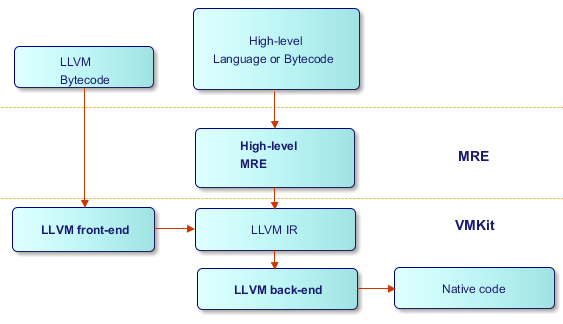
\includegraphics[width=80mm]{vmkitcompilation.png}
\caption{Compilation process in VMKit}
\label{fig:vmkitimplementation}
\end{figure}

\subsection{The JIT Compiler}

The LLVM Project is a collection of modular and reusable compiler and tool chain technologies. All the libraries including VMKit have been implemented in C++. As VMKit is a substrate for VMs, the components integrated in order to develop VMKit should have a general purpose interfaces and functionalities. Therefore the compiler should have support for a general purpose instruction set to allow VMs to implement intermediate representations of arbitrary functions. LLVM JIT is exactly a suitable compiler for this task because of its inherent behavior without  imposing object model or type system.\\
Once the VM generates the intermediate representation (IR) with the help of interfaces provided by LLVM, that VM delegates the compilation to LLVM JIT to generate the native code. LLVM JIT optimizes all methods to the same degree without considering the frequency of the number of time each method get called. This behavior is called the compilation without adaptive optimization. As a result, the initialization time get higher and the runtime also shows some slowness.\\
The LLVM IR is made up five instructions (i) arithmetic, copy and cast operations on registers, (ii) local control flow instructions (branch), (iii) method invocation (direct and indirect), (iv) memory reads and writes and (v) intrinsics.\\

\begin{figure}[ht!]
\centering
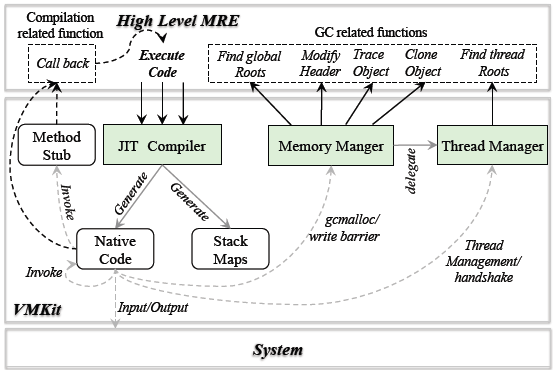
\includegraphics[width=80mm]{vmkit.png}
\caption{VMKit architecture}
\label{fig:vmkitimplementation}
\end{figure}

\subsection{Compiler extension with  intrinsics}
Any language should be able to map to the LLVM IR. Since LLVM directly targets the C language, there are many instructions that are not extensible in C that could be used by MREs, e.g. atomic instructions. LLVM supports this instructions by means of intrinsics: an intrinsic is a contract between the language and the compiler to generate a specific assembly instruction. It is materialized as a function call in LLVM. Beside atomic instructions there are other processor instructions, like vector operations, math operations and stack operations that LLVM implement as intrinsics.

\subsection{Lazy Compilation}
The execution engine performs lazy compilation of the methods throughout the lifetime of the application i.e. in case a method calls another method which has not been translated or compiled yet, the execution engine inserts a callback. When called, the callback invokes the high-level MRE method to locate the new method.The high-level MRE provides the callback function. It loads and generates the intermediate representation of the lazily compiled function, and finally delegates to LLVM the generation of its native representation. Once the function is generated, LLVM patches the calling site to call the newly generated function for subsequent calls.